%++++++++++++++++++++++++++++++++++++++++
% Don't modify this section unless you know what you're doing!
\documentclass[letterpaper,12pt]{article}
\usepackage{tabularx} % extra features for tabular environment
\usepackage{amsmath}  % improve math presentation
\usepackage{amssymb}
\usepackage{graphicx} % takes care of graphic including machinery
\usepackage[margin=1in,letterpaper]{geometry} % decreases margins
\usepackage{cite} % takes care of citations
\usepackage[final]{hyperref} % adds hyper links inside the generated pdf file
\usepackage{float}
\usepackage[toc,page]{appendix}
\usepackage{listings}
\usepackage{siunitx}
\usepackage{pdfpages}
\usepackage{fancyhdr}
\usepackage{caption}
\usepackage{booktabs}
\usepackage{algorithm,algpseudocode}




\setlength{\parskip}{1em}
\setlength\parindent{0pt}


\hypersetup{
	colorlinks=true,       % false: boxed links; true: colored links
	linkcolor=blue,        % color of internal links
	citecolor=blue,        % color of links to bibliography
	filecolor=magenta,     % color of file links
	urlcolor=blue
}


\newcommand{\degrees}{^\circ}
\newcommand{\di}{\partial}
%++++++++++++++++++++++++++++++++++++++++

\title{Design of a PID Auto-Tuner for an Automatic Levelling Wrist}
\author{}
\date{\today}											% Date

\makeatletter
\let\thetitle\@title
\let\theauthor\@author
\let\thedate\@date
\makeatother

\pagestyle{fancy}
\fancyhf{}
\rhead{\theauthor}
\lhead{\thetitle}
\cfoot{\thepage}


\begin{document}

\begin{titlepage}
	\centering
    \vspace*{-1 cm}
    
\includegraphics[scale = 0.5]{UW.jpg}\\	% University Logo
    \textsc{\Large Department of Mechanical and Mechatronics Engineering}\\[2.0 cm]
	\rule{\linewidth}{0.2 mm} \\[0.4 cm]
	{ \huge \bfseries \thetitle}\\
	\rule{\linewidth}{0.2 mm} \\[1.5 cm]

	\begin{minipage}[t]{0.4\textwidth}
		\begin{flushleft} \large
			\emph{Author:}\\
            James Graham-Hu \\
			\end{flushleft}
			\end{minipage}~
			\begin{minipage}[t]{0.4\textwidth}
			\begin{flushright} \large
			\emph{Student Number:} \\
				20555690 \\
		\end{flushright}
	\end{minipage}\\[2 cm]
	Date:
	{\large \thedate}\\[2 cm]
	\vfill

\end{titlepage}
%%%%%%%%%%%%%%%%%%%%%%%%%%%%%%%%%%%%%%%%%%%%%%%%%%%%%%%%%%%%%%%%%%%%%%%%%%%%%%%%%%%%%%%%%
\pagenumbering{gobble}
\thispagestyle{empty}
%%letter of submittal
\thedate\\

William Melek, Director\\
Mechatronics Engineering\\
University of Waterloo\\
Waterloo, Ontario\\
N2L 3G1\\

Dear Professor Melek,\\

This report entitled "Title", was prepared as my Work Report 400 for the Department of Mechanical and Mechatronics Engineering at the University of Waterloo for the 4A term. Purpose of report.\\

Description of Amii.\\

Description of project and motivation behind project.\\


Thank yous.
This report was written entirely by  me and has not received any previous academic credit at this or any other institution.\\

Sincerely,\\

James Graham-Hu\\
ID 20555690\\
4A Mechatronics Engineering



\pagebreak
%%%%%%%%%%%%%%%%%%%%%%%%%%%%%%%%%%%%%%%%%%%%%%%%%%%%%%%%%%%%%%%%%%%%%%%%%%%%%%%%%%%%%%%%%
\pagenumbering{roman}
\tableofcontents
% \setcounter{page}{1}
\pagebreak
\listoffigures
\pagebreak
\listoftables
\pagebreak


%%%%%%%%%%%%%%%%%%%%%%%%%%%%%%%%%%%%%%%%%%%%%%%%%%%%%%%%%%%%%%%%%%%%%%%%%%%%%%%%%%%%%%%%%
\pagenumbering{arabic}
\section{Summary}
Summary
\pagebreak
\section{Introduction}
\subsection{Problem Definition}
Demos can provide an interesting and intuitive way to demonstrate the capabilities and advantages of machine learning to interested parties. Although a few software demos exist at Amii, there is currently no demo that implements machine learning on a hardware system. The advantage of implementing machine learning on hardware is that it is a hands-on way of demonstrating how machine learning can improve a system or be applied to a problem. The problem this project addresses is the lack of a hardware demo to demonstrate machine learning at Amii.

\subsection{Objective}
The automatic levelling wrist, developed by Dylan A. J. Brenneis as part of his Master's thesis in 2019, \cite{d.j.a.brenneis} is a good candidate for a hardware system that can be improved with machine learning. The objective of this project is to use machine learning to improve the automatic levelling wrist in a meaningful and  demonstrable way.


\section{Background}
\subsection{Automatic Levelling Wrist Background}
Powered wrist movement is rare in commercial systems, and many powered protheses have only one degree of freedom (DOF), usually rotation \cite{n.m.bajaj}. These limitations in ease of wrist movement in many upper limb prostheses force people with major upper limb loss to use compensatory movements \cite{s.l.carey}. Compensation occurs with trunk, shoulder, and elbow movements, and has been associated with causing musculoskeletal pain in the neck, upper back, shoulder, and remaining arm \cite{k.ostlie}.

A two DOF automatic levelling wrist was developed by Dylan J. A. Brenneis in 2019 that addresses the issues with ease of wrist movement in wrist prosthetics \cite{d.j.a.brenneis}. The two DOF automatic levelling wrist provides two degrees of freedom, rotation and flexion of the wrist. The user has the ability to switch between controlling the position of the flexion, or letting it automatically level itself to maintain its angle with the ground (see figure \ref{fig:auto_levelling}). The rotation of the wrist is always automatically leveled to be flat with the ground. These features are shown to reduce compensatory movements in vertically-oriented tasks. However, the current implementation of the automatic levelling wrist is reported as unreliable and unintuitive in user tests \cite{d.j.a.brenneis}. Possible reasons for a feeling of unreliability from users could be a result of slow response time, oscillations, and poor disturbance rejection in the automatic levelling system.

\begin{figure}[H]
\centering 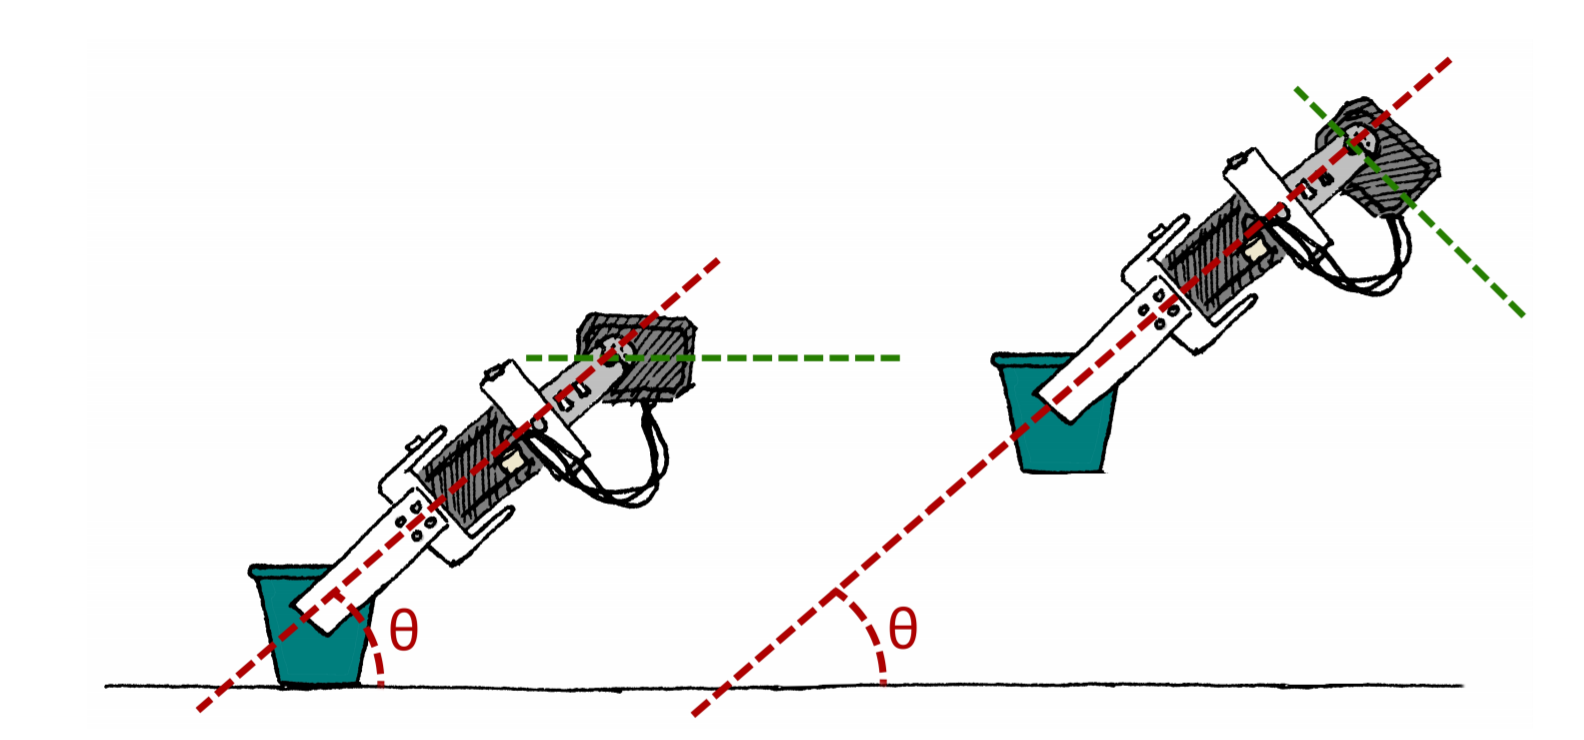
\includegraphics[width=0.8\columnwidth]{auto_levelling.png}
\caption{\label{fig:auto_levelling}Automatic levelling of the flexion. The angle, $\theta$, of the flexion servo is constant with the ground as the arm moves (represented by the green dashed line) \cite{d.j.a.brenneis}.}
\end{figure}

Figure \ref{fig:slw_diagram} shows the design of the automatic levelling wrist. Three MX-28AT servos are used to actuate the prosthetic wrist. Two servos provide the degrees of freedom for wrist rotation and flexion, and the third servo is used to manipulate a gripper. It should be noted that the automatic levelling wrist is designed as a bypass protheses so that an able-bodied person is able to use it. A higher statistical power is able to be achieved in a more time efficient way by running trials with able-bodied persons, because of limitations in participant availability when running trials with participants affected by amputation \cite{d.j.a.brenneis}.

\begin{figure}[H]
\centering 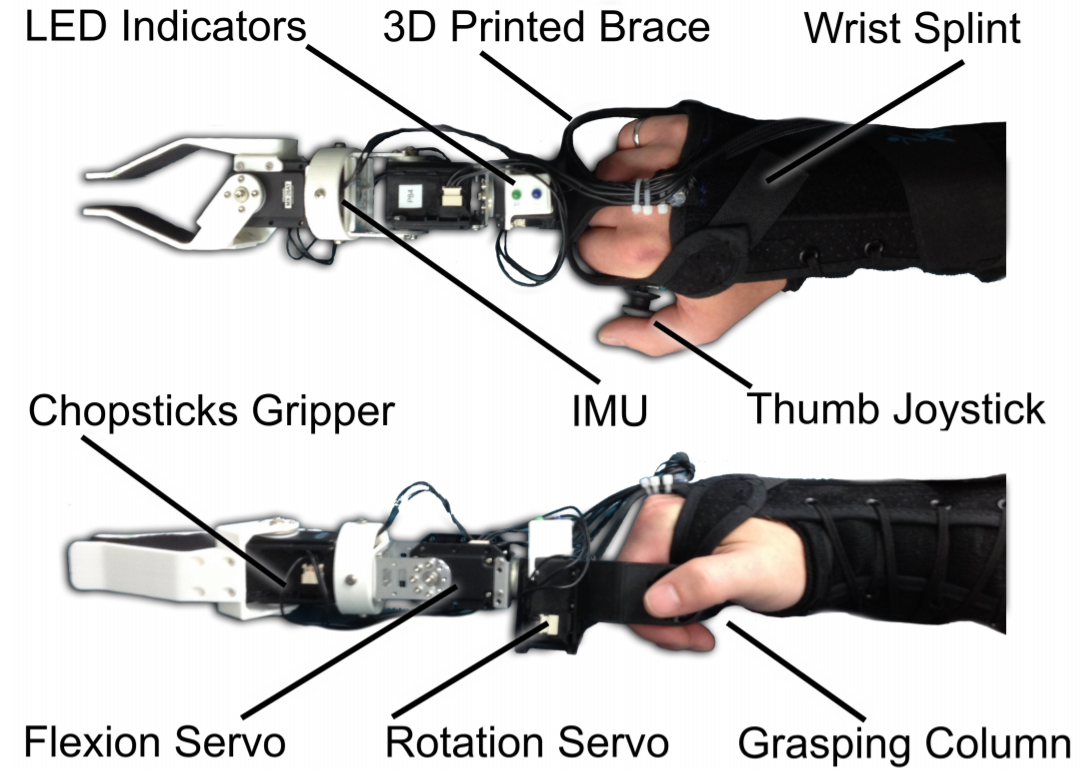
\includegraphics[width=0.8\columnwidth]{slw_diagram.png}
\caption{\label{fig:slw_diagram}Diagram of the automatic levelling wrist bypass protheses \cite{d.j.a.brenneis}.}
\end{figure}

\subsubsection{Automatic Levelling Method}
The wrist is automatically leveled using an Adafruit 9-DOF absolute orientation IMU fusion breakout (BNO055) attached to the base of the gripper, as seen in figure \ref{fig:slw_diagram}, and two independent PID controllers, one for the rotation servo and one for the flexion servo. The gravity vector from the IMU is used to calculate the current angle of rotation and flexion. The error between the calculated angle and the setpoint is fed into the PID controller to generate a control signal for the servo. The setpoint for the rotation servo is always set to $180\degrees$ while the setpoint for the flexion servo is set to where the user last moved it to before switching to automatic levelling. Figure \ref{fig:angles} shows the definitions for the coordinate system, the angle of rotation, $\phi$, and the angle of flexion, $\theta$.

\begin{figure}[H]
\centering 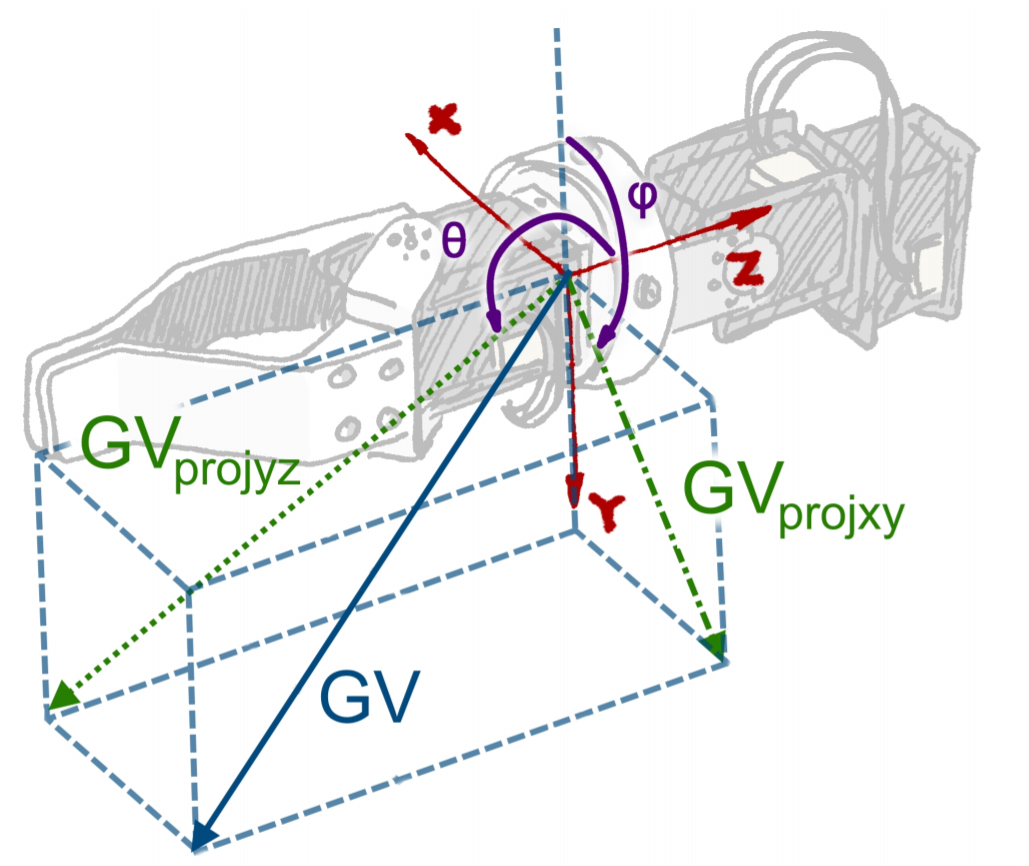
\includegraphics[width=0.8\columnwidth]{angles.png}
\caption{\label{fig:angles}Coordinate system and angles, $\phi$ and $\theta$. The projections of the IMU gravity vector (GV) can be used to calculate $\phi$ and $\theta$ \cite{d.j.a.brenneis}.}
\end{figure}

$\phi$ is defined as the angle between the negative y-axis and the projection of the gravity vector in the x-y plane. $\theta$ is defined as the angle between the positive z-axis and the projection of the gravity vector projected in the y-z plane.

Figure \ref{fig:servo_system} shows the block diagram for one servo in the automatic levelling wrist. A simple PID control loop controls the position of the servo. The equation for the PID controller signal, $u(t)$, is given by equation \ref{eq:pid}. The servo position is summed with a disturbance, $d(t)$ which models the angle the wrist is rotated by the user, and fed through the IMU to acquire either $\phi$ or $\theta$. The block diagram for the rotation and flexion servos are the same other than the $K_p$, $K_i$, and $K_d$ gain values for the PID controllers, the IMU function, and the value of the disturbance, $d(t)$. The disturbance is considered as the angle of the user's wrist with respect to a fixed coordinate system that is coincident with the user's wrist when it is completely level with the ground. Note that in the actual implementation of the control loop, the disturbance and servo position aren't directly used. Rather, they are implicitly included when the IMU measures the gravity vector since the gravity vector changes based on the disturbance and servo positions.

\begin{equation}
	\label{eq:pid}
	u(t) = K_p e(t) + K_i \int e(t) dt + K_d \frac{de(t)}{dt}
\end{equation}

\begin{figure}[H]
\centering 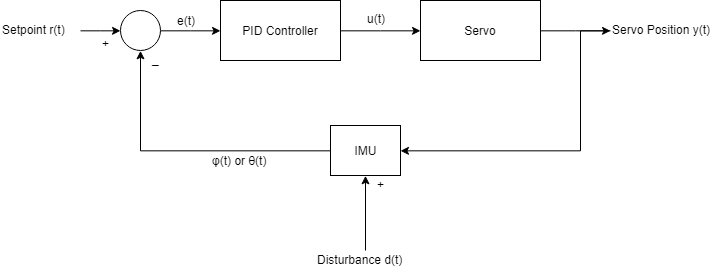
\includegraphics[width=0.8\columnwidth]{servo_system.png}
\caption{\label{fig:servo_system}Block diagram of the control loop for one servo.}
\end{figure}

\subsection{Neural Network Background}
In machine learning, neural networks are used to represent non-linear functions by making use of one or more hidden layers and activation functions. Figure \ref{fig:nn} shows the structure of a neural network with one hidden layer. In this network, the input vector, $X$, is multiplied by the weight matrix $W_{0}$ and summed with the bias vector $b_{0}$. The result of that is then put through an activation function, giving a vector of activations. These activations are then multiplied by the weight matrix $W_{1}$ and summed with the bias vector $b_{1}$ to give the output, $y$. The output can also be put through an activation function. In regression, a linear activation function is mostly used on the output. Activation functions used in the hidden layer include but are not limited to the hyperbolic tangent, sigmoid, and rectified linear unit (ReLU) functions. The choice of activation function is dependent on the application of the neural network.

\subsubsection{Backpropagation}
Learning for a neural network is most commonly accomplished by backpropagation. Backpropagation is performed by calculating the derivative of the squared error of the neural network with respect to each weight in the network. The squared error of the neural network is defined in equation \ref{eq:sq_error}. The equation is divided by two to simplify the derivative. Since the entire network including its activation functions is differentiable, the chain rule can be used to backpropagate the error between the neural network's output and what the output should be (the label) back to the weights. Equation \ref{eq:nn_equation} is the update function used for weight $w_{i,j}$ in the neural network which updates the weights at a learning rate $\alpha$.

\begin{equation}
	\label{eq:sq_error}
	E = \frac{1}{2}(y_{true} - y_{pred})^2
\end{equation}

\begin{equation}
	\label{eq:nn_equation}
	w_{i, j} \leftarrow w_{i,j} + \alpha \frac{\di E}{\di w_{i, j}}
\end{equation}

\subsubsection{Levenberg-Marquardt Algorithm}\label{sec:levenberg}
Another method for training neural networks is using the Levenberg-Marquardt algorithm. The Levenberg-Marquardt algorithm uses the jacobian of the output with respect to the weights of the neural network to solve for an adjustment for each weight. Equation \ref{eq:levenberg} is solved for $\sigma$ to determine the adjustments for each weight.

\begin{equation}
	\label{eq:levenberg}
	[J_w^T J_w + \lambda I]\sigma = J_w^T [E]
\end{equation}
Here, $J_w$ is the jacobian of the output with respect to the weights, $\lambda$ is the damping factor, $I$ is the identity matrix, $\sigma$ is the adjustment matrix, and $E$ is the difference between the outputs and the labels. Isolating for $\sigma$ yields equation \ref{eq:levenberg_solved}. The damping factor, $\lambda$, is increased if $[J_w^T J_w + \lambda I]$ is not invertible. Once $\sigma$ is acquired, it is added to the previous weights to move them closer to the optimal values. This process is repeated iteratively until the weights converge.


\begin{equation}
	\label{eq:levenberg_solved}
	\sigma = [J_w^T J_w + \lambda I]^-1 J_w^T [E]
\end{equation}

For a system, $y(\bf{u_i}, w)$ with one output, an input vector, $\bf{u_i}$, $n$ timesteps, and $k$ weights, the jacobian with respect to the neural network weights is expressed as equation \ref{eq:jacobian}.

\begin{equation}
	\label{eq:jacobian}
	J_w = \begin{bmatrix}
		\frac{\di y(\bf{u_0}, \bf{w})}{\di w_0} & \frac{\di y(\bf{u_0}, \bf{w})}{\di w_1} & \cdots & \frac{\di y(\bf{u_0}, \bf{w})}{\di w_k} \\
		\frac{\di y(\bf{u_1}, \bf{w})}{\di w_0} & \frac{\di y(\bf{u_1}, \bf{w})}{\di w_1} & \cdots & \frac{\di y(\bf{u_1}, \bf{w})}{\di w_k} \\
		\vdots & \vdots & \ddots & \vdots \\
		\frac{\di y(\bf{u_n}, \bf{w})}{\di w_0} & \frac{\di y(\bf{u_n}, \bf{w})}{\di w_1} & \cdots & \frac{\di y(\bf{u_n}, \bf{w})}{\di w_k}


	\end{bmatrix}
\end{equation}

\subsubsection{Numerically Calculating the Jacobian of the Servo}\label{sec:numerical_jacobian}
To numerically calculate jacobian of a servo, each weight is individually changed by a small amount, $\epsilon$ and then an input signal is sent to the servo. The change in servo response before and after the small weight change is recorded and used to calculate a finite backward difference to approximate the partial derivative of the system with respect to the weight that was changed. Equation \ref{eq:jacobian_numerical_calc} demonstrates this calculation of the approximate jacobian matrix. The dimension of the resultant jacobian matrix is $n$ rows by $k$ columns.

\begin{equation}
\begin{split}
	\label{eq:jacobian_numerical_calc}
	& J_w = \begin{bmatrix}
		\frac{\di \bf{y}(\bf{u}, \bf{w})}{\di w_0} & \frac{\di \bf{y}(\bf{u}, \bf{w})}{\di w_1} & ... & \frac{\di \bf{y}(\bf{u}, \bf{w})}{\di w_k}
	\end{bmatrix} \\
	& \frac{\di \bf{y}(\bf{u}, \bf{w})}{\di w_i} = \frac{\bf{y}(\bf{u}, \bf{w}) - \bf{y}(\bf{u}, \bf{w} - \bf{h}\epsilon(w_i))}{\epsilon(w_i)} \\
	& h_p = 1, p = i \\
	& h_p = 0, p \neq i
\end{split}
\end{equation}

\subsection{Amplitude Modulated Pseudo-Random Binary Signal}
An amplitude modulated pseudo-random binary signal (APRBS) can be used to excite a system such that all frequencies are excited equally \cite{o.nelles}. The signal approximates the spectrum and statistical properties of	white noise, as it has a mean of one and variance of zero. The signal is also deterministic, making it consistent between trials. The method used to generate an APRBS in this project is outlined in Johannes Günther's paper \cite{j.gunther}. Figure \ref{fig:aprbs} is an example of an APRBS with a maximum amplitude of 1, 500 step length, and maximum hold time of 100 steps. The orange signal is the same APRBS with a first order butterworth filter applied to make the edges less "sharp".

\begin{figure}[H]
\centering 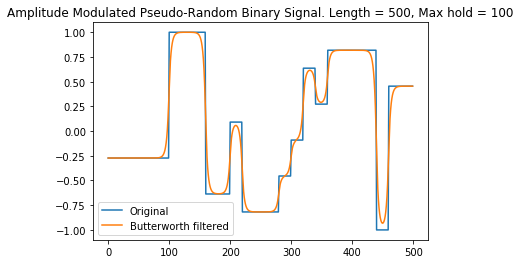
\includegraphics[width=0.8\columnwidth]{aprbs.png}
\caption{\label{fig:aprbs}APRBS with a maximum amplitude of 1, 500 step length, and maximum hold time of 100 steps. With and without first order butterworth filter.}
\end{figure}

% \subsection{Reinforcement Learning Background}
% Reinforcement learning is a machine learning method based on an agent interacting with its environment. The agent takes actions within the environment, which leads to a new state within the environment and a reward for the action. Figure \ref{fig:rl_diagram} describes the interaction between the agent and the environment it exists in.
% The goal of the agent is to maximize the expected, cumulant of discounted future rewards by taking the best action for the situation, or state, that the agent is in. Equation \ref{eq:rl_basic} formally shows what the agent is maximizing.
%
% \begin{equation}
% \begin{split}
% 	\label{eq:rl_basic}
% 	& R_t = \sum_{k=0}^{\infty}\gamma^kr_{t+k+1} \\
% 	& r:S \times A \rightarrow R \\
% 	& \pi: S \rightarrow A \\
% \end{split}
% \end{equation}
%
% $R_t$ is the cumulative reward at time step $t$. $r$ is the reward function that returns a scalar reward based on the action chosen by the agent from the set of possible actions $S$ and the state that the agent was in from the set of possible states $S$. $\pi$ is called the policy. The policy is the function that the agent uses to choose an action given a state. $\gamma \epsilon[0, 1]$ is a scalar value that determines the "far-sightedness" of the agent. If $\gamma=0$ the agent will only see the reward from the next time step. As $\gamma \rightarrow 1$ the agent will look farther into the future.
%
% \begin{figure}[H]
% \centering 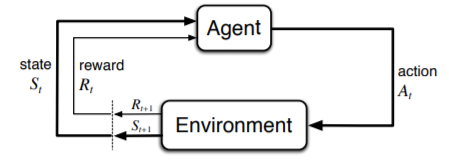
\includegraphics[width=0.8\columnwidth]{rl_diagram.png}
% \caption{\label{fig:rl_diagram}Interaction between an agent and the environment it exists in \cite{r.s.sutton}.}
% \end{figure}
%
% \subsubsection{Q-Learning}
% Q-Learning involves learning an action-value function, $Q(S, A)$, which maps states and actions to a value $Q$. To learn the action-value function, an iterative update is used as shown in equation \ref{eq:q_update}
%
% \begin{equation}
% 	\label{eq:q_update}
% 	Q(s_t, a_t) = (1-\alpha_t) Q(s_t, a_t) + \alpha_t [R_{t+1} + \gamma max_a Q(s_{t+1}, a_{t+1})]
% \end{equation}
%
% At each time step the Q-value for the previous state-action pair, $s_t$ and $a_t$, is updated at a learning rate, $\alpha_t$, by the sum of the received reward, $R_t$, and the discounted Q-value of the next state, $s_{t+1}$, maximized by selecting action $a_{t+1}$. The simplest way to represent the action-value function is to tabulate the values, with each row representing a possible state, and each column representing a possible action. By initializing the table randomly and then letting the agent act according to its policy, $\pi$, the agent can learn the Q-values for each element of the table.
%
% A simple policy that can be used for Q-Learning is the $\epsilon$-greedy policy. With this policy, the agent will either take the action that maximizes its current action-value function, $Q_t$, given its current state, or take a random action from the set of possible actions. The possibility that the agent takes a random action is determined by a the value $\epsilon$, where $0<\epsilon<1$. A higher value of $\epsilon$ means the agent explores more, while a lower value of $\epsilon$ means the agent exploits its current knowledge more. If $\epsilon=0$ the agent will always try to maximize its current action-value function and will not try new actions, which could potentially result in higher rewards. If $\epsilon=1$ the agent will always act randomly, which is useless in most cases. There is always a trade-off between exploitation and exploration, but certain tricks can be used to maximize reward, such as decreasing the exploration rate, $\epsilon$, as time passes and the agent learns to take optimal actions.
%
% \subsubsection{Function Approximation}
% Although tabulated Q-Learning is simple, many problems cannot be described in a discrete way. Function approximation provides a way to model the action-values in a continuous state space using a learned function. Most commonly, the Q function is represented by a neural network that takes the state as its input, and outputs a vector of the action-values for each action in the discrete action space. The update function shown in equation \ref{eq:func_approx} is similar to the tabular case, but uses the difference between the current Q-value and the next reward plus the next Q-value as the error term in the backpropagation for the neural network.
%
% \begin{equation}
% \begin{split}
% 	\label{eq:func_approx}
% 	& E = [R_{t+1} + \gamma max_a Q(s_{t+1}, a_{t+1})] - Q(s_t,a_t) \\
% 	& w_{i,j} \leftarrow w_{i,j} + \alpha_t \frac{\di E}{\di w_{i,j}}
% \end{split}
% \end{equation}


\section{Proposed Solutions}
\subsection{Criteria and Constraints}

The proposed solutions for the project were constrained according to the following constraints.
\begin{itemize}
		\item The solution must improve the performance of the automatic levelling wrist.
    \item The solution must implement machine learning in some way.

\end{itemize}

The following criteria considered in choosing an appropriate solution are chosen such that the automatic levelling wrist reliably improves the user's ability to use the prosthetic.
\begin{itemize}
    \item The solution should minimize steady state error.
		\item The solution should minimize response time.
		\item The solution should minimize settling time.
		\item The solution should maximize reliability and consistency.
\end{itemize}
Due to the nature of the problem, training time and data are difficult to acquire. Without a simulation, data and training can only be collected and run in real time. Therefore, the solution should require minimal training time and data, or be able to make use of a simulation.


\subsection{Neural Network Methods}
The three neural network methods proposed in this section make use of the PID control loop described in Figure \ref{fig:servo_system}. A neural network that outputs the PID gains, $K_p$, $K_i$, and $K_d$ is added to the control loop. The neural network takes the error between the setpoint and the current angle of the servo, the current angle  of the servo, and the velocity of the servo. The goal is to train the neural network so that it will output appropriate gains for any situation, such that the system has the best response time and error for that situation. The rotation and flexion servos will use separately trained neural networks to output gains for their respective PID controllers. In this section the rotation servo will be used to explain the method, but the same method can be applied to both rotation and flexion servos.

\subsubsection{PID Auto-Tuning, Trained Model-Free using Backpropagation}\label{sec:model_free_backprop}
Since no labels exist for the PID gains at the output of the neural network (it is unknown what the gains should be in any given situation) the error term used to train the neural network, $E$, must be the squared error between the servo angle, $\phi(t)$ and the setpoint, $r(t)$ as shown in equation \ref{eq:model_free_error}. To train the neural network, this error must be backpropagated through the servo and the PID controller to the neural network output, $\bf{m}$. Performing the chain rule on the partial derivative of $E$ with respect to $\bf{m}$ yields \ref{eq:backprop_servo}. This partial derivative can then be backpropagated through the neural network to train the weights.

\begin{equation}
	\label{eq:model_free_error}
	E = \frac{1}{2}(r - \phi)^2
\end{equation}

\begin{equation}
	\label{eq:backprop_servo}
	\frac{\di E}{\di \bf{m}} =
	\begin{bmatrix}
		\frac{\di E}{\di \phi} \frac{\di \phi}{\di u} \frac{\di u}{\di K_p} \\
		\frac{\di E}{\di\phi} \frac{\di \phi}{\di u} \frac{\di u}{\di K_i} \\
		\frac{\di E}{\di \phi} \frac{\di \phi}{\di u} \frac{\di u}{\di K_d}
	\end{bmatrix}
\end{equation}

Here, $\phi$ is the rotation servo angle, $u$ is the control signal from the PID controller defined in equation \ref{eq:pid}, and $K_p$, $K_i$, and $K_d$ are the PID gains. The solutions to the individual partial derivatives are shown in equation \ref{eq:partial_derivs}

\begin{equation}
\begin{split}
	\label{eq:partial_derivs}
	& \frac{\di E}{\di \phi} = r - \phi \\
	& \frac{\di \phi}{\di u} = ? \\
	& \frac{\di u}{\di K_p} = e(t) \\
	& \frac{\di u}{\di K_i} = \int e(t)dt \\
	& \frac{\di u}{\di K_d} = \frac{de(t)}{dt} \\
\end{split}
\end{equation}

Since the time domain function of the servo, $\phi(t)$ is not known, it is not possible to solve for $\frac{\di \phi}{\di u}$. To address this problem, a second neural network that mimics the servo is used to output the servo angle rather than the actual servo. This allows the error to be backpropagated through the neural network, through the PID controller and to the PID neural network. Figure \ref{fig:pid_model_free_backprop} is the control loop block diagram with the added PID neural network and servo neural network. The servo neural network will be trained on the actual response of the servo. By treating the input to the servo as the input to the neural network, and the output of the servo as the labels for training, backpropagation can be performed to train the servo neural network on a dataset of inputs and outputs given by the actual servo. Figure \ref{fig:servo_nn_training} demonstrates the training process for the servo neural network. Once trained, the servo neural network is implemented into the control loop to train the PID neural network using backpropagation. After training the PID neural network, the PID neural network is implemented into the actual system.

\begin{figure}[H]
\centering 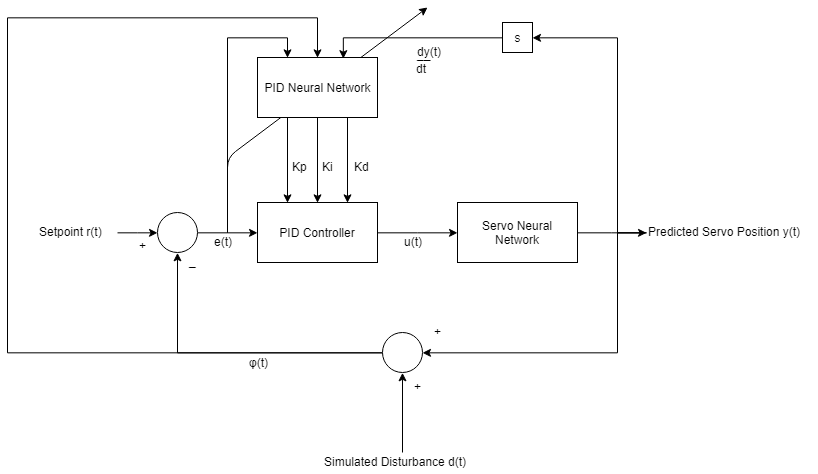
\includegraphics[width=0.8\columnwidth]{pid_model_free_backprop.png}
\caption{\label{fig:pid_model_free_backprop}Block diagram of the training process for the PID neural network using the servo neural network to mimic the actual servo output.}
\end{figure}

\begin{figure}[H]
\centering 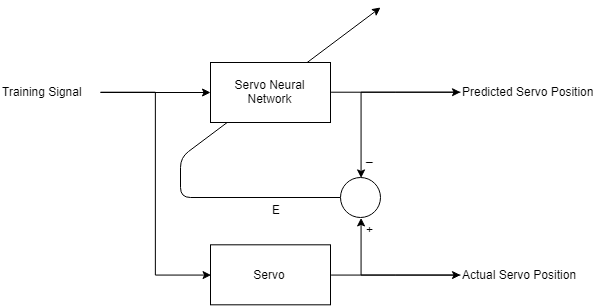
\includegraphics[width=0.8\columnwidth]{servo_nn_training.png}
\caption{\label{fig:servo_nn_training}Block diagram of the training process for the servo neural network.}
\end{figure}


\subsubsection{PID Auto-Tuning, Trained Model-Free using the Levenberg-Marquardt Algorithm}\label{sec:levenberg_model_free}
Rather than using backpropagation to train the weights of the PID neural network, the Levenberg-Marquardt algorithm is used to train the PID neural network as described in section \ref{sec:levenberg}. Equation \ref{eq:levenberg_model_free} is used to solve for the weight adjustments, $\sigma$, using the difference between the servo angle, $\phi$, and the setpoint, $r$, as the error term. A servo neural network, trained the same way as described in \ref{sec:model_free_backprop} is used to simulate the servo response to small weight changes needed to calculate the jacobian of the servo outlined in section \ref{sec:numerical_jacobian}.

\begin{equation}
	\label{eq:levenberg_model_free}
	\sigma = [J_w^T J_w + \lambda I]^-1 J_w^T [\phi - r]
\end{equation}

\subsubsection{PID Auto-Tuning, Trained with a Model using the Levenberg-Marquardt Algorithm}
Similar to section \ref{sec:levenberg_model_free} this method uses the Levenberg-Marquardt algorithm the train the PID neural network. However, when numerically calculating the jacobian, rather than using a neural network to simulate the servo response to small weight changes, a mathematical model of the servo is used. Equation \ref{eq:servo_tf} is the simplified transfer function of the servo, assuming the electrical dynamics of the servo are much faster than the mechanical dynamics \cite{m.r.o.a.maximo}.

\begin{equation}
	\label{eq:servo_tf}
	\frac{Y(s)}{U(s)} = \frac{N \eta K_t (K_d s^2 + K_p s + K_i)}{R (J_l + J_m N^2 \eta)s^3 + (b_m N^2 \eta R + \frac{K_t N^2 \eta}{K_\omega} + N \eta K_t K_d)s^2 + N \eta K_t K_p s + N \eta K_t K_i}
\end{equation}

Here, $Y(s)$ is the laplace transform of the servo angle, $U(s)$ is the laplace transform of the input signal.
The MX-28AT servo contains an internal PID controller with internal gains. Since the servo is controlled in ticks rather than radians, the gains must be converted so that they can be used in the transfer function which is in radians. Equation \ref{eq:internal_gains_conversion} shows the conversion process.

\begin{equation}
\begin{split}
	\label{eq:internal_gains_conversion}
	& K_p = \frac{P}{8} \frac{2048 V_s}{511 \pi} \\
	& K_i = \frac{1000 I}{2048} \frac{2048 V_s}{511 \pi} \\
	& K_d = \frac{4 D}{1000} \frac{2048 V_s}{511 \pi} \\
\end{split}
\end{equation}

Here, $V_s$ is the source voltage which is $12 V$, and $P$, $I$, and $D$ are gains set by the user, which are $P=32$, $I=0$, and $D=0$ by default. The user manual for the MX-28AT also states that the gains set by the user must be converted to get their values in ticks, hence the multiplication by $\frac{1}{8}$, $\frac{1000}{2048}$ and $\frac{4}{1000}$ for $P$, $I$, and $D$ respectively \cite{robotis}.

The load inertia, $J_l$, depends on the servo. For the rotation servo the inertia is estimated as the inertia of a rectangular prism, which represents the flexion servo, rotating on its center axis, and a point mass, which represents the gripper, whose position above the axis of rotation depends on the angle of the flexion servo. For the flexion servo the inertia is estimated as the inertia of a rectangular prism, which represents the gripper, rotating around an axis offset from its center by half its length and the length of the bracket attaching the gripper to the flexion servo. Although these assumptions oversimplify the inertia, the load inertia, $J_l$, is relatively small compared to the other term, $J_mN^2\eta$, in the $s^3$ term of the denominator ($J_l$ is on an order of magnitude of $10^-4$ and $J_mN^2\eta$ is on an order of magnitude of $10^-3$). Therefore, any error incurred due to these assumptions will be small. The inertia calculations are shown in equation \ref{eq:inertia}.

\begin{equation}
\begin{split}
	\label{eq:inertia}
	& J_{l, rot} = m \frac{b^2 + h^2}{12} + (l + c)^2 sin(\theta)^2 \\
	& J_{l, flex} = m (d^{2/3} + d l + l^2)
\end{split}
\end{equation}

Here, $m$, is the mass of the MX-28AT servo, $b$ is the width of the servo, $h$ is the height of the servo, $d$ is the depth of the servo, $l$ is the length of the bracket connecting the gripper to the flexion servo, and $c$ is the center of mass of the gripper.


The other parameters for equation \ref{eq:servo_tf} are described in table \ref{tab:servo_params}.

\begin{table}[H]
	\begin{center}
		\caption{Parameters for the MX-28AT servo model \cite{m.r.o.a.maximo}}
        \label{tab:servo_params}
        \begin{tabular}{l|l|l}
        Parameter & Symbol & Value \\
        \hline
				Motor resistance & $R$ & $8.3 \Omega$ \\
				Motor gear ratio & $N$ & $193$ \\
				Motor gear efficiency & $\eta$ & $0.836$ \\
				Speed constant & $K_{\omega}$ & $93.1 rad/V$ \\
				Torque constant & $K_t$ & $0.0107 Nm/A$ \\
				Motor inertia & $J_m$ & $8.68 \times 10^{-8} kgm^2$ \\
				Friction & $b_m$ & $8.87 \times 10^{-8} Nms$ \\
        \end{tabular}
	\end{center}
\end{table}

To account for voltage saturation of the power supply at $12V$, the input signal is saturated so that it doesn't exceed this limit. As an initial guess, the saturation limit is set to $10\degrees$. This means that the control signal, $u(t)$, is saturated at $-10\degrees$ and $10\degrees$.

Figure \ref{fig:pid_model_levenberg} is the control loop block diagram with the PID neural network and the servo model for training. Once training of the PID neural network is complete, the neural network weights can be used to generate the PID gains for the actual servo in the physical implementation.


\begin{figure}[H]
\centering 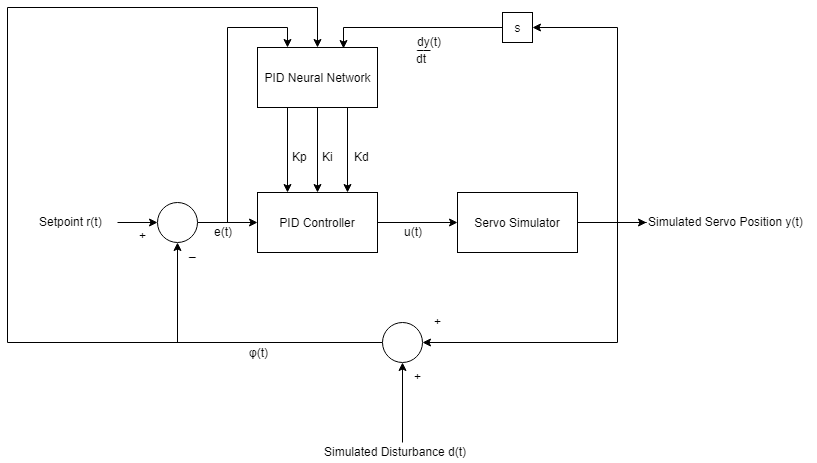
\includegraphics[width=0.8\columnwidth]{pid_model_levenberg.png}
\caption{\label{fig:pid_model_levenberg}Block diagram of the training process for the PID neural network using the servo model.}
\end{figure}


% \subsection{Reinforcement Learning Methods}
% Tabular Q-learning
% Q-learning with function approximation


\section{Solution Evaluation}
Judging the three proposed solution methods without implementing them shows that they each have the potential to improve the performance of the automatic levelling wrist according to the criteria. The deciding factor is the amount of data needed to train each solution method. For the model-free methods, the methods that use the servo neural network, real servo data is needed. Although servo data can be recorded and reused, many data points are needed to train the neural network in order for the neural network to learn the servo's time-domain function. A neural network is trained on a 8000 data point training set and its performance is tested on a 2000 data point test set. The training and test data consist of an APRBS with a maximum amplitude of $\frac{\pi}{2}$ radians as the input, and the actual servos output as the label. Data is collected at a rate of 5ms per time step. Figure \ref{fig:model_results_1} shows that the neural network's prediction on the test set is close to the actual servo.

\begin{figure}[H]
\centering 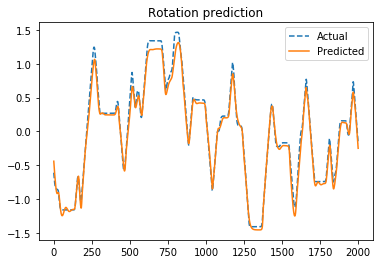
\includegraphics[width=0.8\columnwidth]{model_results_1.png}
\caption{\label{fig:model_results_1}Actual and predicted servo position for APRBS with a maximum amplitude of $\frac{\pi}{2}$ over 2000 time steps, at 5ms per time step.}
\end{figure}

Figure \ref{fig:model_results_2} shows the results of testing the neural network on a $\frac{\pi}{2}$ step input. While the response somewhat resembles what the actual servo's response, it does not perfectly track the input.

\begin{figure}[H]
\centering 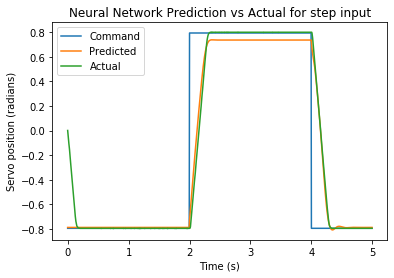
\includegraphics[width=0.8\columnwidth]{model_results_2.png}
\caption{\label{fig:model_results_2} Neural network prediction vs actual for the step input.}
\end{figure}

These problems could potentially be rectified by using more training data. However, the results for the mathematical model are promising, without the need to collect data. Figure \ref{fig:simulation_results_1} shows the same test as the one ran on the neural network model. It shows that the mathematical model can closely simulate the servo.

\begin{figure}[H]
\centering 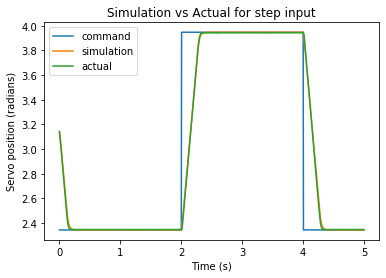
\includegraphics[width=0.8\columnwidth]{simulation_results_1.png}
\caption{\label{fig:simulation_results_1}Simulation vs actual for the step input.}
\end{figure}

Since no data is needed for mathematical model and the mathematical model can closely simulate the actual servo, the chosen solution method is PID auto tuning trained with a model using the Levenberg-Marquardt algorithm.
% \subsection{Q-learning - Tabular}
% Tabular control wasn't granular enough to enable precise control of the servo
% Even with a minimized state space (only using the IMU angle), it was still difficult to visit all states and learn making it unreliable.
% \subsection{Q-learning - Function Approximation}
% Not enough data to train the neural network, difficult to visit all states, no simulation (must train real-time which is very slow especially if testing different hyperparameters)
% Deadly triad (bootstrapping, function approximation and off-policy learning) - not guaranteed to converge

\section{PID Auto-Tuning Implementation}
The control software for the automatic levelling wrist is implemented in C\# \cite{blincdev}. However, Python provides a better environment for machine learning. First, Python is used for training the PID neural network. Then after the neural network is trained, the weights are copied into an identical neural network in the C\# control code.

\subsection{Simulation Implementation}
The method used to simulate the servo from the servo's mathematical model is SciPy's odeint function \cite{odeint}. This function receives an initial state, an array of timesteps, and an ordinary differential equation (ODE). The ODE is found by computing the inverse Laplace transform of the servo's transfer function. Equation \ref{eq:ode} is the ODE for the servo.

\begin{equation}
	\label{eq:ode}
	\ddot y(t) = \frac{- b_m N^2 \eta R - \frac{K_t N^2 \eta}{K_\omega + N \eta K_t K_d}}{R(J_l + J_m N^2 \eta)} \dot y(t) + \frac{-N \eta K_t K_p}{R(J_l + J_m N^2 \eta)} y(t) + \frac{N \eta K_t K_p}{R(J_l + J_m N^2 \eta)} u(t)
\end{equation}

To better simulate the actual servo, an angle sampling delay, $a_{angle}$, and a control signal delay, $a_{control}$, are  implemented into the simulation. This is because the angle reading from the actual IMU, and the reaction from the servo to a control signal from the PID controller can be delayed. The delays are mathematically described in equation \ref{eq:delays}.

\begin{equation}
\begin{split}
	\label{eq:delays}
	& \phi_{delayed}(t) = \phi(t - a_{angle}) \\
	& u_{delayed}(t) = u(t - a_{control})
\end{split}
\end{equation}

To tune the simulation to match the actual servo, a grid search over a parameter space for the time step length, angle sampling delay, saturation, and control delay, is performed. For each parameter combination, the response of the simulation is compared to the actual servo's response to a step response. The parameter combination with the lowest root-mean-squared error when compared to the actual response is chosen as the best parameter combination. Figure \ref{fig:paramcombo} compares the servo response to a step input for the actual servo and the simulation with the best parameters. Table \ref{tab:bestparams} shows the best parameters from the grid search.

\begin{figure}[H]
\centering 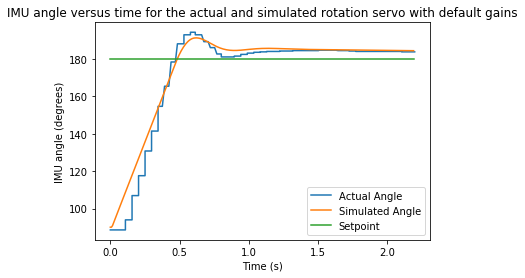
\includegraphics[width=0.8\columnwidth]{paramcombo.png}
\caption{\label{fig:paramcombo}Tuned simulation vs actual for a step input.}
\end{figure}

\begin{table}[H]
	\begin{center}
		\caption{Best Parameters for the Simulation}
        \label{tab:bestparams}
        \begin{tabular}{l|l|l}
					\hline
        	Time step length & $dt$ & $0.04$ s \\
					Angle sampling delay & $a_{angle}$ & $3$ time steps \\
					Saturation point & $s$ & $8.789 \degrees$ \\
					Control sampling delay & $a_{control}$ & $0$ time steps \\
        \end{tabular}
	\end{center}
\end{table}


Algorithm \ref{alg:simulation} shows how Figure \ref{fig:pid_model_levenberg} is implemented in code to run a simulation. Here, $T$ is the number of timesteps, each with a length $dt$, $t_i$ is the time at timestep $i$, $r(t)$ is the setpoint in degrees, $d(t)$ is the disturbance in degrees, $y(t)$ is the angle of the servo in radians, $\phi(t)$ is the IMU angle in degrees, $e(t)$ is the error between the setpoint and the IMU angle, $u(t)$ is the control signal in degrees, $y_0$ and $\dot y_0$ are the initial conditions of the servo. $\phi(t)$ is defined such that when $y(t) = \SI{0}{rad}$ and $d(t) = 0\degrees$, the servo angle is $\phi(t)=180\degrees$. This is consistent with how the servo angle is defined in figure \ref{fig:angles}.

\begin{algorithm}
	\caption{Servo Simulation}\label{alg:simulation}
	\begin{algorithmic}[1]
		\State Input: $T$, $r(t)$, $d(t)$, $y_0$, $\dot y_0$.
		\State Output: $\phi(t)$.
		\For{$i = 0$ to $T$}
			\State $e(t_i) = r(t_i) - \phi(t_{i-1-a_{control}})$
			\Comment Get error with delayed angle sample.

			\State $\dot y (t_{i-1}) =\frac{y(t_{i-1}) - y(t_{i-2})}{t_{i-1} - t_{i-2}}$
			\Comment Calculate velocity with first backwards difference.

			\State $K_p, K_i, K_d =$ Get\_Gains($e(t_i), \phi(t_{i-1}), \dot y(t_{i-1})$)
			\Comment Predict the PID gains with the PID neural network.

			\State PID.Set\_Gains($K_p, K_i, K_d$)
			\State $u(t_i) = $PID.Get\_Control\_Signal($e(t_i)$)
			\Comment Get control signal.

			\State $u_{delay} = u(t_{i-a_{angle}})$
			\Comment Get delayed control signal.
			\State $u_{delay\_sat} = $min(max($u_{delay}, -s$), $s$)
			\Comment Saturate the control signal.

			\State $\dot y_0, y_0 = $SciPy.odeint($\dot y_0, y_0, [t_{i-1}, t_i], u_{delay\_sat}$)
			\Comment Run odeint for one timestep.
			\State $\phi(t_i) = y_0 \frac{180}{\pi} + 180 + d(t_i)$
			\Comment Calculate $\phi$ by adding disturbance and $180 \degrees$.
		\EndFor
		\State \Return $\phi$
		\Comment Return time response of the servo.
	\end{algorithmic}
\end{algorithm}

\subsection{PID Neural Network Training}
The PID neural network is trained using the Levenberg-Marquardt algorithm. Algorithm \ref{alg:training} describes this process \cite{e.reichensdorfer}. Here, the values are the same as in algorithm \ref{alg:simulation}. For training, $d(t)$ is an APRBS signal with length $25.0 s$, peak-to-peak amplitude of $45 \degrees$ and maximum hold time of $5.0s$. $x$ starts at 200 samples, and increases by 200 for each trial. 10 trials are run in total. The best weights are chosen from the 10 trials, according to which weights yield the lowest root mean squared error (RMSE) between the servo angle and the setpoint. Because the difference in load inertias for the rotation servo and flexion servo is small, it is assumed that the neural network will work similarly for both servos, so the same weights can be used for both servos.

\begin{algorithm}
	\caption{Servo Simulation}\label{alg:training}
	\begin{algorithmic}[1]
		\State Input: $T$, $r(t)$, $d(t)$, $y_0$, $\dot y_0$.
		\State Output: Trained PID Neural Network Weights $\bf{w}$.
		\While{Trials left}
			\State Perform truncated random initialization for neural network weights, $\bf{w}$.
			\State $T_{tmp}=T(t_0 ... t_x),r_{tmp}=r(t_0 ... t_x), d_{tmp}=d(t_0 ... t_x)$
			\Comment Sample first $x$ values of $T$, $r$, and $d$.
			\While{Not converged}
				\State $J_w = $Compute\_Jacobian($T$, $r(t)$, $d(t)$, $y_0$, $\dot y_0$)
				\Comment Numerically Compute jacobian using equation \ref{eq:jacobian_numerical_calc} and simulation from algorithm \ref{alg:simulation}.
				\State $\phi_{sim}$ = Simulate($T$, $r(t)$, $d(t)$, $y_0$, $\dot y_0$)
				\Comment Simulate servo response.

				\State $\sigma = [J_w^T J_w + \lambda I]^-1 J_w^T [\phi_{sim} - r]$
				\Comment Solve Levenberg-Marquardt equation for $\sigma$.

				\If{RMSE for simulation with  $\bf{w} + \sigma <$ RMSE for simulation with $\bf{w}$}
					\State $\bf{w} \leftarrow \bf{w} + \sigma$
					\State $\lambda = \frac{\lambda}{2}$
				\Else
					\State $\lambda = 2\lambda}$
				\EndIf

			\EndWhile
			\If{RMSE for simulation with $\bf{w} < $ RMSE for simulation with $\bf{w}_{best}$}
				\State $\bf{w}_{best} \leftarrow \bf{w}$
				\State Increase number of samples, $x$.
			\EndIf
		\EndWhile
		\State \Return $\bf{w}_{best}$
	\end{algorithmic}
\end{algorithm}


\subsection{Neural Network Structure}
The structure of the neural network is shown in figure \ref{fig:nn_structure}. The neural network structure consists of 5 input nodes, 4 hidden nodes, and 3 output nodes. The input nodes consist of normalized error, normalized angle, normalized velocity, and activation values from hidden nodes 2 and 3. Normalization is performed using equation \ref{eq:normalization} which scales the inputs to a value between 0 and 1. Normalization is important, as it ensures the scale of each input value is equal relative to each other, so no single input can "overshadow" the other inputs \cite{}. The activation values from hidden nodes 2 and 3 are used to give the network a one time-step recurrence, which can aid in applications of temporal nature such as a control system \cite{j.gunther}.

\begin{equation}
	\label{eq:normalization}
	x_{normalized} = \frac{x - x_{min}}{x_{max} - x_{min}}
\end{equation}

\begin{figure}[H]
\centering 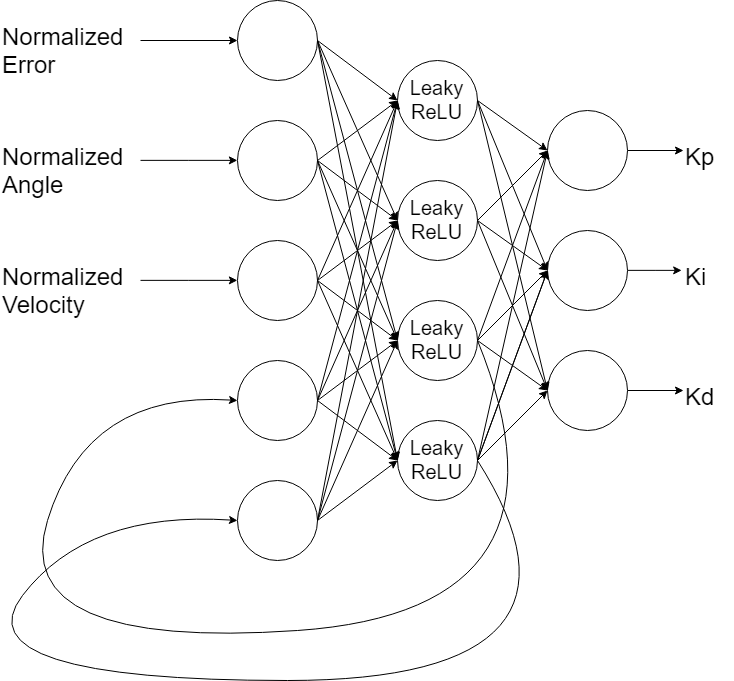
\includegraphics[width=0.8\columnwidth]{nn_structure.png}
\caption{\label{fig:nn_structure}Structure of the PID neural network.}
\end{figure}

The activation function used at the hidden layer is a leaky ReLU with a slope of $0.3$. Equation \ref{eq:leakyrelu} is the equation describing a leaky ReLU.

\begin{equation}
	\label{eq:leakyrelu}
	a = \[ \begin{cases}
      0.3z & z\leq 0 \\
      z & z > 0
			\end{cases}
	 \]
\end{equation}

\section{Results}
The PID neural network training was performed for the rotation servo for 10 trials using the APRBS shown in figure \ref{fig:aprbs_train}. The best trial was trial three, which yielded an RMSE of $22.034$ on the training APRBS.

\begin{figure}[H]
\centering 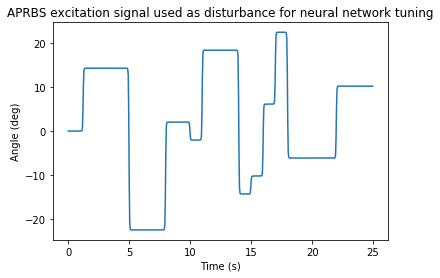
\includegraphics[width=0.8\columnwidth]{aprbs_train.png}
\caption{\label{fig:aprbs_train}APRBS used for training.}
\end{figure}

After training, the neural network weights were copied into the PID neural network for both the rotation servo and the flexion servo in the C\# program. A test was run to compare the step response of the automatic levelling wrist with and without PID Auto-Tuning. Figure \ref{fig:rotation_results} show the results of this test for the rotation servo. Figure \ref{fig:rotation_gains} shows the value of the gains at each step in the test. Table \ref{tab:rmse_results} is the RMSE values for the rotation and flexion servo step response with and without PID auto-tuning. Analyzing figure \ref{fig:rotation_results} and figure \ref{fig:flexion_results} shows that PID auto-tuning can reduce the response time of the system, while also reducing overshoot and oscillations. RMSE was decreased by approximately $30\%$ for both the rotation and flexion servos when PID auto-tuning was used.

\begin{table}[H]
	\begin{center}
		\caption{RMSE Values for Step Responses}
        \label{tab:rmse_results}
        \begin{tabular}{l|l|l}
					& w/o PID Auto-Tuning & w/ PID Auto-Tuning \\
					\hline
        	Rotation & $1383.64$ & $995.86$ \\
					Flexion & $1553.36$ & $1027.76$ \\
        \end{tabular}
	\end{center}
\end{table}

\begin{figure}[H]
\centering 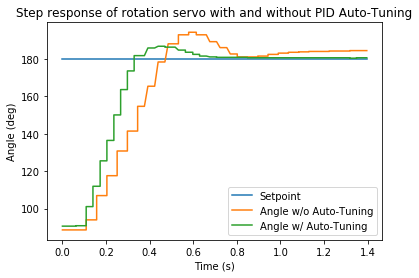
\includegraphics[width=0.8\columnwidth]{rotation_results.png}
\caption{\label{fig:rotation_results}Rotation servo step response with and without PID Auto-Tuning.}
\end{figure}

\begin{figure}[H]
\centering 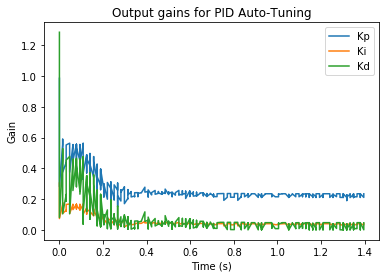
\includegraphics[width=0.8\columnwidth]{rotation_gains.png}
\caption{\label{fig:rotation_gains}PID gains output by the rotation PID neural network during the step response test.}
\end{figure}

\begin{figure}[H]
\centering 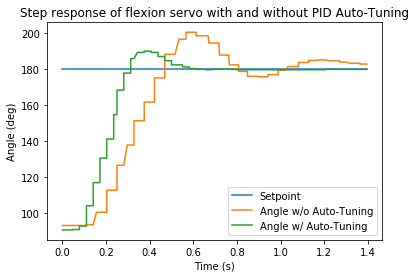
\includegraphics[width=0.8\columnwidth]{flexion_results.png}
\caption{\label{fig:flexion_results}Flexion servo step response with and without PID Auto-Tuning.}
\end{figure}

\begin{figure}[H]
\centering 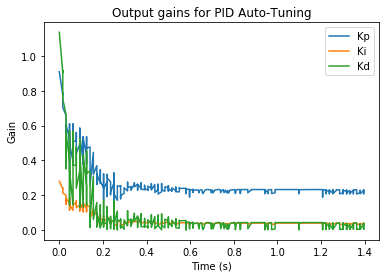
\includegraphics[width=0.8\columnwidth]{flexion_gains.png}
\caption{\label{fig:flexion_gains}PID gains output by the flexion PID neural network during the step response test.}
\end{figure}


\section{Conclusion}
From the results it can be seen that PID auto-tuning can significantly improve the performance of the automatic levelling wrist. PID auto-tuning shows an RMSE decrease of approximately $30\%$ for both servos, as well as reduced response time, overshoot and oscillations. Figure \ref{fig:rotation_gains} and figure \ref{fig:flexion_gains} show how the neural network acts in reaction to a disturbance. First the neural network increases the gains of $K_p$ and $K_i$, to increase response time and tracking. Then as the servo moves closer to the setpoint, the PID gains are decreased to more stable values so that overshoot and oscillations are reduced.

From the results it can also be seen that the consequences of sharing weights between the rotation and flexion servos do not greatly affect the performance of the PID auto-tuning network, as the performance of the rotation and flexion servos are on par with each other.

In conclusion, PID auto-tuning for the automatic levelling wrist provides a tangible demo to show how machine learning can significantly improve the performance of a hardware system.

\section{Recommendations}
Although the PID auto-tuner can improve the performance of the automatic levelling wrist there is room for improvement.

The training process can be improved to include more trials as well as variations in the neural network structure. More trials would increase the chance that a good initialization is found, as initialization is random. Trying different neural network structures such as changing number of nodes, changing activation functions, and changing which node is recurrent could lead to an increase in performance, as the structure proposed in this project is not known to be optimal.

The position of the flexion servo can affect the response of the rotation servo because the load moment of inertia changes depending on the position of the flexion servo. A similar problem arises when a load is applied to the gripper, as the added load will increase the load moment of inertia for the rotation and flexion servos. These changing moments of inertia are not considered in the simulation and as a results the PID neural network is not trained to handle these situations. To address this problem the neural network should include the flexion servo position and sensed load in its inputs (the MX-28AT servos have load sensors). To supplement this, training should include situations with varying loads so that it can learn to adapt to these differing situations.

With these improvements and with further tuning of the simulation parameters, PID auto-tuning can greatly improve the performance of the automatic levelling wrist so that it is more reliable, and more intuitive for users to use.
\pagebreak

\begin{thebibliography}{99}
\bibitem{n.m.bajaj}
N. M. Bajaj, A. J. Spiers, and A. M. Dollar, “State of the art in prosthetic wrists: Commercial and research devices”, in \textit{2015 IEEE International Conference on Rehabilitation Robotics
(ICORR)}, Aug. 2015, pp. 331–338.

\bibitem{s.l.carey}
S. L. Carey, M. J. Highsmith, M. E. Maitland, and R. V. Dubey, “Compensatory movements
of transradial prosthesis users during common tasks”, \textit{Clinical Biomechanics}, vol. 23, no. 9,
pp. 1128 –1135, 2008.

\bibitem{k.ostlie}
K. Østlie, R. J. Franklin, O. H. Skjeldal, A. Skrondal, and P. Magnus, “Musculoskeletal pain
and overuse syndromes in adult acquired major upper-limb amputees”, \textit{Archives of Physical
Medicine and Rehabilitation}, vol. 92, no. 12, pp. 1967 –1973, 2011.

\bibitem{d.j.a.brenneis}
D. J. A. Brenneis, "Automatic Levelling of a Prosthetic Wrist", \textit{University of Alberta}, 2019.

\bibitem{o.nelles}
O. Nelles, "Nonlinear system identification, Classical approaches to neural networks and fuzzy models", \textit{Berlin, Heidelberg: Springer Verlag}, 1 ed., 2010

\bibitem{j.gunther}
J. Gunther, "Machine intelligence for adaptable closed loop and open loop production engineering systems", \textit{University of Alberta}, 2019.

\bibitem{r.s.sutton}
R. S. Sutton and A. G. Barto, "Introduction to reinforcement learning", Dissertation, \textit{Technische Universität München}, Munich, Germany, 2018.

\bibitem{m.r.o.a.maximo}
M. R. O. A. Maximo, C. H. C. Ribeiro and R. J. M. Afonso, "Modeling of a position servo used in robotics applications", \textit{Autonomous Computational Systems Lab (LAB-SCA) and Electronic Engineering Division, Computer Science Division, Aeronautics
Institute of Technology, Pra¸ca Marechal Eduardo Gomes}, 2017.

\bibitem{robotis}
"Robotis e-manual", \textit{Robotis}, 2019. [Online]. Available: http://emanual.robotis.com/docs/en/dxl/mx/mx-28/. [Accessed: 16-Jul-2019].

\bibitem{blincdev}

\bibitem{odeint}
https://docs.scipy.org/doc/scipy/reference/generated/scipy.integrate.odeint.html

\bibitem{e.reichensdorfer}
% \bibitem{whatisacodec}
% "What is a CODEC? And why is it an important component of videoconferencing?", \textit{Jwhornvideoconference.com}, 2018. [Online]. Available: http://www.jwhornvideoconference.com/what-is-a-codec-and-why-is-it-an-important-component-of-videoconferencing. [Accessed: 16- Aug- 2018].
%
% \bibitem{s3}
% "Cloud Object Storage", \textit{Amazon Web Services, Inc.}, 2018. [Online]. Available: https://aws.amazon.com/s3/. [Accessed: 16- Aug- 2018].
%
% \bibitem{ec2}
% "Amazon EC2", \textit{Amazon Web Services, Inc.}, 2018. [Online]. Available: https://aws.amazon.com/ec2. [Accessed: 16- Aug- 2018].
%
% \bibitem{lambda}
% "AWS Lambda – Serverless Compute", \textit{Amazon Web Services, Inc.}, 2018. [Online]. Available: https://aws.amazon.com/lambda/. [Accessed: 16- Aug- 2018].
%
% \bibitem{dynamodb}
% "Amazon DynamoDB", \textit{Amazon Web Services, Inc.}, 2018. [Online]. Available: https://aws.amazon.com/dynamodb/. [Accessed: 16- Aug- 2018].
%
% \bibitem{firewall}
% "What is firewall? - Definition from WhatIs.com", \textit{SearchSecurity}, 2018. [Online]. Available: https://searchsecurity.techtarget.com/definition/firewall. [Accessed: 16- Aug- 2018].
%
% \bibitem{querystring}
% "What is a Query String?", \textit{Techopedia.com}, 2018. [Online]. Available: https://www.techopedia.com/definition/1228/query-string. [Accessed: 16- Aug- 2018].
%
% \bibitem{uuiddef}
% P. Leach, M. Mealling and R. Salz, "RFC 4122 - A Universally Unique IDentifier (UUID) URN Namespace", \textit{Tools.ietf.org}, 2005. [Online]. Available: https://tools.ietf.org/html/rfc4122\#section-4.2. [Accessed: 16- Aug- 2018].
%
% \bibitem{uuidunique}
% "Are UUIDs really unique?", \textit{Towards Data Science}, 2018. [Online]. Available: https://towardsdatascience.com/are-uuids-really-unique-57eb80fc2a87. [Accessed: 16- Aug- 2018].
%
% \bibitem{uuidunique2}
% "Advanced", \textit{2database.com}, 2018. [Online]. Available: http://www.h2database.com/html/advanced.html\#uuid. [Accessed: 16- Aug- 2018].
%
% \bibitem{statuscode}
% "HTTP/1.1: Status Code Definitions", \textit{W3.org}, 2018. [Online]. Available: https://www.w3.org/Protocols/rfc2616/rfc2616-sec10.html. [Accessed: 16- Aug- 2018].
%
% \bibitem{mvc}
% "MVC Framework Introduction", \textit{www.tutorialspoint.com}, 2018. [Online]. Available: https://www.tutorialspoint.com/mvc\_framework/mvc\_framework\_introduction.htm. [Accessed: 16- Aug- 2018].
%
% \bibitem{https}
% "What is HTTPS?", \textit{Techopedia.com}, 2018. [Online]. Available: https://www.techopedia.com/definition/5361/hypertext-transport-protocol-secure-https. [Accessed: 16- Aug- 2018].
%
%

\end{thebibliography}

\begin{appendices}
\section{Appendix}
\end{appendices}


\end{document}
